Similar to the previous years, this year’s tournament challenges too involved various non-verbal user interactions such as detecting an object the user was pointing to. In the previous section, we explained our approach to recognizing people in 3D. 
Once the recognition results are inserted into the world model, additional properties can be added to the people taking other entities in the world model into account, e.g. “\emph{is\_pointing\_at\_entity}”. This information is used by the top-level state machines to implement challenges such as `Hand Me That', the description of which can be found in the 2019 Rulebook\footnote{\url{http://www.robocupathome.org/rules}}. However an additional check based on spatial queries is inserted to ensure that the correct operator is found. By using such a query it is possible to filter out people based on their location. Finally, to determine at which entity the operator is pointing to, we implemented ray-tracing, as illustrated in Figure \ref{fig:ray_trace}.

\begin{figure}[H]
	\centering
    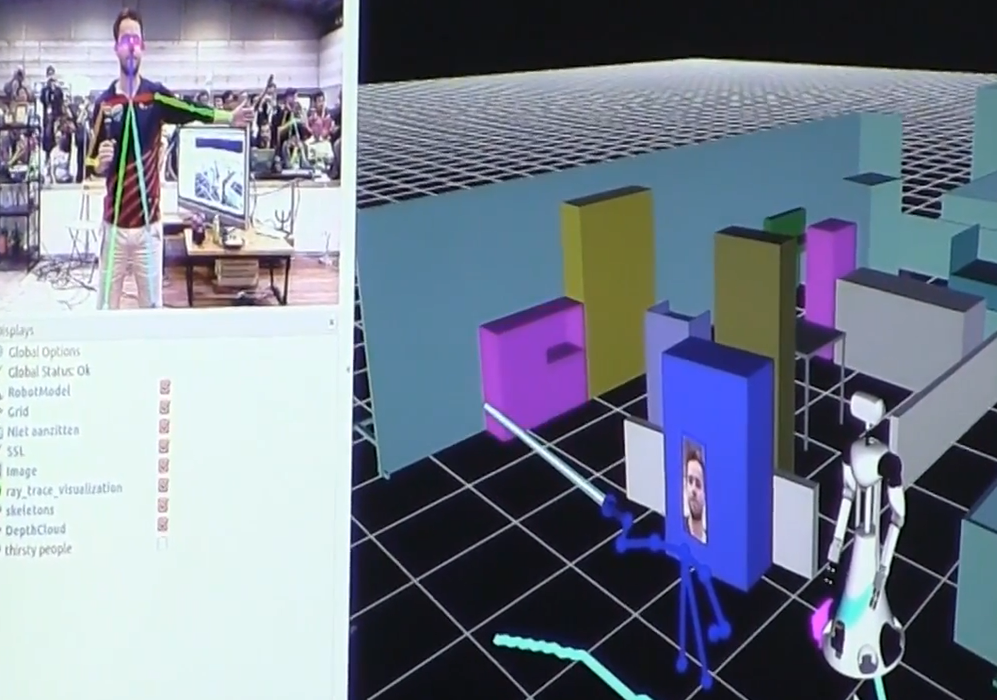
\includegraphics[width=0.6\linewidth]{ed_ray_trace2}
	\caption{Ray-tracing based on pose detection with AMIGO.}
	\label{fig:ray_trace}
\end{figure}


